%  report.tex
%  Document created by seblovett on seblovett-Ubuntu
%  Date created: Tue 01 Apr 2014 19:44:08 BST
%  <+Last Edited: Fri 04 Apr 2014 16:41:25 BST by hl13g10 on octopus +>

\documentclass[12pt]{article}

\usepackage[nodayofweek]{datetime}
\usepackage{graphicx}
\usepackage{todonotes}
\usepackage{multirow} 
\usepackage{listings}
\usepackage{amsmath}
\usepackage{color}
\usepackage{booktabs}
\author{Henry Lovett \\ hl13g10 \\ MEng Electronic Engineering \\ Tutor: Prof. Mark Zwolinski}

\title{ELEC6016 - FPGA Synthesis of a picoMIPS}

%TC:macro \todo 1
\begin{document}
\maketitle
\listoftodos
\begin{abstract}
\todo[inline]{Abstract: Summarise your work in less than 100 words stating briefly what was achieved.}
This report documents the design and test of a picoMIPS processor.
The processor is able to calculate an affine transform with predefined constants. 
A small instruction set of ten instructions was implemented with an eight bit opcode format. 
The processor is a register-accumulator based architecture. 
\end{abstract}
%TC:ignore



\definecolor{mygreen}{rgb}{0,0.6,0}
\definecolor{mygray}{rgb}{0.5,0.5,0.5}
\definecolor{mymauve}{rgb}{0.58,0,0.82}

%Code Styles
\lstset{basicstyle=\scriptsize\ttfamily,
  backgroundcolor=\color{white},   % choose the background color; you must add \usepackage{color} or \usepackage{xcolor}
  basicstyle=\footnotesize,        % the size of the fonts that are used for the code
  breakatwhitespace=false,         % sets if automatic breaks should only happen at whitespace
  breaklines=true,                 % sets automatic line breaking
  captionpos=t,                    % sets the caption-position to bottom
  commentstyle=\color{mygreen},    % comment style
  deletekeywords={...},            % if you want to delete keywords from the given language
  escapeinside={\%*}{*)},          % if you want to add LaTeX within your code
  extendedchars=true,              % lets you use non-ASCII characters; for 8-bits encodings only, does not work with UTF-8
  frame=single,                    % adds a frame around the code
  keepspaces=true,                 % keeps spaces in text, useful for keeping indentation of code (possibly needs columns=flexible)
  numbers=left,                    % where to put the line-numbers; possible values are (none, left, right)
  numbersep=5pt,                   % how far the line-numbers are from the code
  numberstyle=\tiny\color{mygray}, % the style that is used for the line-numbers
  rulecolor=\color{black},         % if not set, the frame-color may be changed on line-breaks within not-black text (e.g. comments (green here))
  showspaces=false,                % show spaces everywhere adding particular underscores; it overrides 'showstringspaces'
  showstringspaces=false,          % underline spaces within strings only
  showtabs=false,                  % show tabs within strings adding particular underscores
  stepnumber=1,                    % the step between two line-numbers. If it's 1, each line will be numbered
  tabsize=2,                       % sets default tabsize to 2 spaces
  title=\lstname                   % show the filename of files included with \lstinputlisting; also try caption instead of title
}
\lstdefinestyle{sverilog} {
  language=Verilog,
  otherkeywords={always\_ff,always\_comb,assert,logic,return,\$random,\#*},            % if you want to add more keywords to the set
  stringstyle=\color{mymauve},     % string literal style
  keywordstyle=\color{blue}      % keyword style
}
\lstdefinestyle{asm} {
  otherkeywords={PASSA,MULT,ADD,STACC,LUI,ADDI,STSW,WAIT0,WAIT1,JMPA},            % if you want to add more keywords to the set
  keywordstyle=\color{blue},       % keyword style
  language={[x86masm]Assembler}                % the language of the code
}

\todo[inline]{Get \# numbers coloured in verilog listings}
%\todo[inline]{Neaten all synthesis figures}
%\todo[inline]{Standardise all tables}
\todo[inline]{Spell Check}

%TC:endignore
%For each:
% Design of
% Test
%  Introduction.tex
%  Document created by seblovett on seblovett-Ubuntu
%  Date created: Tue 01 Apr 2014 19:50:43 BST
%  <+Last Edited: Tue 01 Apr 2014 19:51:11 BST by seblovett on seblovett-Ubuntu +>

\section{Introduction}

State the objectives of the assignment. Summarise briefly your preparation work,  your experimental work,, and results achieved. Specifically, state which parts of the assignment were delivered according to the requirements and summarise any extensions to the basic specification you have carried out with references to the sections.  ( approx. 0.5 page).



%  Architecture.tex
%  Document created by seblovett on octopus
%  Date created: Wed 02 Apr 2014 14:03:33 BST
%  <+Last Edited: Wed 02 Apr 2014 14:28:33 BST by hl13g10 on octopus +>

\section{Architecture}

Discuss the overall architecture


\begin{figure}
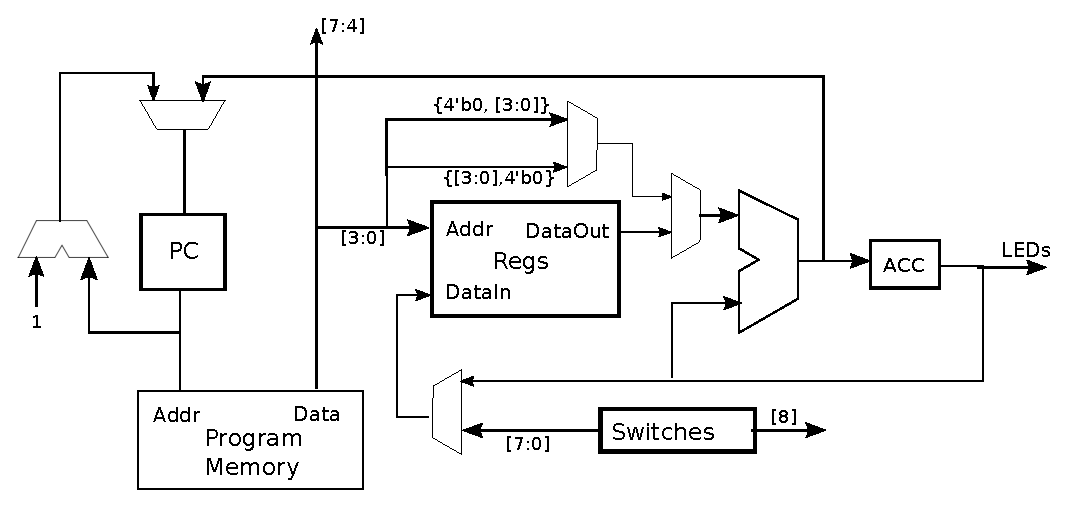
\includegraphics[width=\textwidth]{Figures/architecture.eps}
\caption{Block Diagram of the architecture. Control unit and signals have been omitted for clarity.}
\label{fig:arch}
\end{figure}

% ISA.tex
%  Document created by seblovett on seblovett-Ubuntu
%  Date created: Tue 01 Apr 2014 20:08:47 BST
%  <+Last Edited: Fri 04 Apr 2014 10:07:02 BST by hl13g10 on octopus +>


\section{Instruction Set}

%Discuss what instructions are implemented
In total, ten instructions are implemented in the design.
There are fully documented in table \ref{tab:isa}. 


\begin{table}
\caption{Instruction Set and their operations}
\label{tab:isa}
\begin{tabular}{ccc} \hline 
Instruction & Acronym & Operation \\ \hline
Store Switches & STSW Rn & Rn $\leftarrow$ Switches[7:0] \\
Store Accumulator & STACC Rn & Rn $\leftarrow$ Acc \\
Wait while 0 & WAIT0 & if(Switches[8] == 1) Pc++ \\
Wait while 1 & WAIT1 & if(Switches[8] == 0) Pc++ \\
Absolute Jump & JMPA Imm & PC $\leftarrow$ Acc + Imm \\
Load Upper Immediate & LUI Imm & Acc $\leftarrow$ {Imm, 4'b0000} \\
Add Immediate & ADDI Imm & Acc $\leftarrow$ Acc + Imm \\
Add Register & ADD Rn & Acc $\leftarrow$ Acc + Rn \\
Multiply Register & MULT Rn & Acc $\leftarrow$ Acc * Rn \\
Pass Register & PASSA Rn & Acc $\leftarrow$ Rn \\ \hline
\end{tabular}
\end{table}


\subsection{Arithmetic Instructions}

Only three instructions implemented conduct arithmetic operations, \texttt{ADD}, \texttt{ADDI} and \texttt{MULT}. 
These are all signed arithmetic and are the only functions needed to compute the affine transform. 
\texttt{ADDI} is the addition of an unsigned immediate. 
No subtract immediate instruction was implemented to reduce the size of the ALU and no sign extension is needed for the immediate. 

\subsection{Accumulator and Register Instructions}
%LUI, STSW, STACC, PASSA

The switches provide the main data input to the processor. 
A store switches instruction is implemented to directly store to a register. 
Load upper immediate is used to load constants from the program memory to the accumulator. 
Used in conjunction with the \texttt{ADDI} instruction, any 8 bit value can be loaded to the accumulator in two instructions. 
This can then be used to make a negative number to use for an arithmetic function.

The register-accumulator register, although allows for only one operand, must also include extra instructions to move data.
The instructions needed are a pass to accumulator (\texttt{PASSA}), to write a value from a register to the accumulator, with no modification. 
A store accumulator instruction is also needed to write back the data to a register. 

\subsection{Control Instructions}

The affine transform does not involve any decisions based on the data. 
The only required control flow is during the handshaking protocol. 
As this is reliant on the value of Switches[8], this is accomplished by two instructions, \texttt{WAIT0} and \texttt{WAIT1}. 
These will only allow the program counter to increment if the value of Swithes[8] is correct.
This means no flags need to be used in the design, and no conditional branches. 

An absolute jump is also implemented. 
It is used once the affine transform is complete to return to the start of the loop.
This replaces the value of the program counter with what is stored in the accumulator plus a four bit immediate. 
It means that the processor can jump to any eight bit memory location in two instructions.


\subsection{Instruction Format}

A total of ten instructions have been implemented. 
Combined with the use of a four bit immediate, this lends the instruction set to use an eight bit instruction.
This is summarised in table \ref{tab:instruction}.
A simple instruction format lends itself to simple decoding. 
A maximum of 16 registers (assuming no dummy register) can be used.

\begin{table}
\caption{The instruction format used}
\label{tab:instruction}
\centering
\begin{tabular}{|p{1cm}|p{1cm}|p{1cm}|p{1cm}|p{1cm}|p{1cm}|p{1cm}|p{1cm}|p{1cm}|} \hline
Bit & 7 & 6 & 5 & 4 & 3 & 2 & 1 & 0 \\ \hline
Use & \multicolumn{4}{|c|}{Opcode} & \multicolumn{4}{|c|}{Immediate / Register} \\ \hline
\end{tabular}
\end{table}

%  Controller.tex
%  Document created by seblovett on seblovett-Ubuntu
%  Date created: Tue 01 Apr 2014 20:09:16 BST
%  <+Last Edited: Wed 02 Apr 2014 13:36:22 BST by hl13g10 on octopus +>


\section{Controller}
Lorem Ipsum\dots

Opcode assignments to the instruction set

K maps to show the minimized logic

why a multicycle controller is needed

ASM chart for the controller (or state transition from altera)

Testbench

Simulation Results. 

Synthesis

%  Program.tex
%  Document created by seblovett on seblovett-Ubuntu
%  Date created: Tue 01 Apr 2014 20:09:49 BST
%  <+Last Edited: Fri 04 Apr 2014 13:33:47 BST by hl13g10 on octopus +>

\section{Program}\label{sect:prog}

%\todo[inline]{The program counter, how and why it works}
\subsection{Program Counter}
The program counter is a register storing the address of the current instruction.
It is used to access the program memory to retrieve instructions. 
The implementation involves a six bit write enable register with a multiplexed input. 
The inputs to the multiplexor are the output of the ALU and an incremented value of itself.
The increment is used to progress the program in normal operation, where as the ALU output is used to jump to any location.
Only six bits are used as the program implemented is 46 instructions long. 

\subsection{Program Memory}
The program memory is implemented as read only memory (ROM). 
This means there is no ability to write to the memory.
It is also sequential memory, meaning it takes a clock edge to output the data at the given address. 
This is advantageous as the Cyclone IV has a large amount of synchronous RAM, which is far more efficient that using logic elements.
However, this then requires a multicycle control unit. 

%\todo[inline]{Program itself}
\subsection{Program}

The program is in two sections, the set up and the loop. 
The set up loads all the constants into the registers. 
The loop then conducts the handshaking and the affine transform. 

\subsubsection{Set Up}

The initial part of the program loads in the matrix coefficients into the registers. 
The coefficients of the A matrix are represented by fixed point notation. 
This means that the values must be 128 times bigger than the decimal equivalent.
Listing \ref{lstsetupcode} shows the code to load all the constants to memory.

\lstinputlisting[style=asm,lastline=18,caption={Loading initial constants}label=lstsetupcode]{../Implementation/transform.asm}


\subsubsection{Loop}

An initial handshake is done to load the values of $x_1$ and $y_1$ into memory. 
This is achieved by using the \texttt{WAIT} instructions to control the program flow, and the \texttt{STSW} to write the switches to a memory location. 
The whole process is seen in listing \ref{lsthandshake1}.

\lstinputlisting[style=asm,firstline=19, lastline=24,caption={Handshaking protocol for switch reading},label=lsthandshake1]{../Implementation/transform.asm}


The affine transform is shown in equation \eqref{eq:affine}.
By multiplying the matrix out, $x_2$ and $y_2$ can be calculated by equations \eqref{eq:x2} and \eqref{eq:y2} respectively. 
Listing \ref{lstaffinex} shows the instructions used to calculated $x_2$. 

\begin{equation}\label{eq:affine}
\begin{bmatrix}
x_2 \\
y_2 
\end{bmatrix}
=
\begin{bmatrix}
a_{11} & a_{12} \\
a_{21} & a_{22} 
\end{bmatrix}
\begin{bmatrix}
x_1 \\
y_1
\end{bmatrix}
+
\begin{bmatrix}
b_1 \\
b_2
\end{bmatrix}
\end{equation}

\begin{equation}\label{eq:x2}
x_2 = a_{11} \times x_1 + a_{12} \times y_1 + b_1
\end{equation}

\begin{equation}\label{eq:y2}
y_2 = a_{21} \times x_1 + a_{22} \times y_1 + b_2
\end{equation}


\lstinputlisting[firstline=25, lastline=35,caption={Affine transform for x2},label=lstaffinex,style=asm]{../Implementation/transform.asm}


Once the transform is complete, a second handshake is done to read back the result. 
The program then jumps to the start of the loop, ready for the next calculation. 
This code is seen in listing \ref{lsthandshake2}.

\lstinputlisting[firstline=41, lastline=46,caption={End of loop code to display results and return to the beginning of the loop},style=asm,label=lsthandshake2]{../Implementation/transform.asm}


%\todo[inline]{Talk about assembler too?}
\todo[inline]{Jump locations in asm? Be good to implement. Filling all of memory too? If I'm doing this, .defines also...}
A basic assembler is implemented to aid development.
It is capable of reading the SystemVerilog package containing the definition of the opcodes.
It then assembles the program into the hex values. 
Concurrent development of programs and processor is then greatly simplified as all definitions are obtained from the same package.


The testing of the program counter is done as a part of the datapath test and is discussed in section \ref{sect:datapath}.
%\todo[inline]{Is it possible to test? It is part of the overall datapath.}
%\todo[inline]{synthesis?}
\subsection{Synthesis}

The synthesised logic of the ROM can be seen in figure \ref{fig:ramsynth}.
It shows that there is some redundancy in the logic as the standard cells contain write circuitry.
Here, constants are used to disable the functionality, as these are fabricated, rather than built out of logic elements.


\begin{figure}
\includegraphics[width=\textwidth]{Figures/ramsynth.png}
\caption{Synthesis of the Program ROM module}
\label{fig:ramsynth}
\end{figure}
% and Program Memory
%\input{Program Counter}
%  Registers.tex
%  Document created by seblovett on seblovett-Ubuntu
%  Date created: Tue 01 Apr 2014 20:10:32 BST
%  <+Last Edited: Fri 04 Apr 2014 12:29:48 BST by hl13g10 on octopus +>

\section{Registers}\label{sect:regs}

%\todo[inline]{Design}
The allocation in the instruction set allows for up to 16 general purpose registers. 
In the program, discussed in section \ref{sect:prog}, only 11 registers are used. 
Six are used to store the constants, two for the initial vector, two for the result and a temporary register.
To save RAM, only the required registers are implemented.
This still requires a four bit address and attempting to address the registers above the valid range would result in undefined behaviour.

The registers were implemented using the Synchronous RAM.
This, at the expense of performance, utilised the on chip SRAM blocks. 
The design was parametrised to allow the data and address width and number of registers to be easily changed. 

%\todo[inline]{Explain Test Bench}

\subsection{Testbench}

A task is used to do a basic test.
The code for this task is seen in listing \ref{lstregtask}.
A random byte of data, and a random register are chosen. 
The data is then written to the register. 
The input data is changed to check that the data on the output is stored in memory and assertions are used to verify. 
The data is checked to persist after the write enable signal is inactive. 
If an assertion fails, a global error counter is incremented.

This task is then done a large amount of times to check all registers. 
Figure \ref{fig:regsim} shows the output waveform of the simulation. 
The error count is zero at the end of the simulation showing that the module is functioning correctly.




\lstinputlisting[style=sverilog,firstline=33, lastline=51,caption={Register task for writing and reading to the register.},label=lstregtask]{../Implementation/registers_stim.sv}
%\todo[inline]{Simulation Results}

\begin{figure}
\includegraphics[width=\textwidth,height=\textheight]{Figures/registerssim.eps}
\caption{Waveform simulation for register testbench}
\label{fig:regsim}
\end{figure}

\subsection{Synthesis}
%\todo[inline]{Synthesis}

The synthesised logic of the register module is shown in \ref{fig:registersynth}.
This is virtually identical to the Program ROM module, seen in figure \ref{fig:ramsynth} apart from the write address and data are inputs, rather than hardwired constants.
This utilises the internal SRAM of the FPGA. 

\begin{figure}
\includegraphics[width=\textwidth]{Figures/registersynth.png}
\caption{Synthesis of the register module}
\label{fig:registersynth}
\end{figure}

%  ALU.tex
%  Document created by seblovett on seblovett-Ubuntu
%  Date created: Tue 01 Apr 2014 20:10:56 BST
%  <+Last Edited: Tue 01 Apr 2014 20:11:14 BST by seblovett on seblovett-Ubuntu +>


\section{ALU}
Lorem Ipsum\dots


%  cpu.tex
%  Document created by seblovett on octopus
%  Date created: Thu 03 Apr 2014 12:56:02 BST
%  <+Last Edited: Thu 03 Apr 2014 12:57:14 BST by hl13g10 on octopus +>

\section{Processor}

The whole processor is pulled together in two encapsulating modules. 
The datapath module links the registers and ALU and implements the data multiplexors, program counter and accumulator.
The top level CPU module links the program ROM, controller and datapath. 

\subsection{Datapath}
\todo[inline]{Explain testbench}
\todo[inline]{Simulation Results}
\todo[inline]{Synthesis}

\subsection{CPU}
\todo[inline]{Describe testbench}
\todo[inline]{Full System Test}
\todo[inline]{Full system synthesis}



%  DE0.tex
%  Document created by seblovett on seblovett-Ubuntu
%  Date created: Tue 01 Apr 2014 20:11:21 BST
%  <+Last Edited: Wed 02 Apr 2014 17:38:41 BST by hl13g10 on octopus +>

\section{DE0 Implementation}

\todo[inline]{Use of the slow clock}
\todo[inline]{Demo define to allow for easier use during demo.}
\todo[inline]{Issues encounterd}
\todo[inline]{Synthesised logic. Put some sexy figures in here}


% Implementation

%  Conclusion.tex
%  Document created by seblovett on seblovett-Ubuntu
%  Date created: Tue 01 Apr 2014 20:11:41 BST
%  <+Last Edited: Fri 04 Apr 2014 16:40:45 BST by hl13g10 on octopus +>


\section{Conclusion}

%\todo[inline]{Which objectives in intro have been done. }
The final processor satisfies the specification and the objectives highlighted in section \ref{sect:intro}.
The processor is a register-accumulator based, MIPS-esk \todo{is this an appropriate term?!} architecture. 
It implements ten instructions in total to calculate the affine transform of 8 bit data.

%\todo[inline]{Cost figure}
The total cost of the processor is 72.
A full breakdown of the costs is seen in table \ref{tab:costs}.
A large amount of the cost is located in the datapath. 
This is due to the multiplexors needed to direct the data around. 
A more compact design could be achieved by aiming to minimize these elements. 
The two registers in the datapath also contribute a fair amount to the cost. 
These are a compromise and by using a register-register architecture, the decoding logic is increased and a larger instruction is needed.
Overall, the design is a success, passing thorough testing and achieves the initial goals. 


\begin{table}
\caption{Break down of the costs by module. Costs do not include any instances made by the module. Clock reduction and debugging logic is not included in this cost.}
\label{tab:costs}
\begin{tabular}{cccc} \toprule
Module		& Logic Elements	& Memory (bits)	& Embedded Multipliers \\ \midrule
Control		& 9			& 0		& 0	\\
Datapath	& 24			& 0		& 0	\\
Registers	& 0			& 88		& 0	\\
ALU		& 21			& 0		& 1	\\
ROM		& 0			& 512		& 0 	\\ \midrule
Total 		& 54			& 600		& 1 	\\ \bottomrule
\end{tabular}
\end{table}

%\todo[inline]{General conclusion }




\end{document}

